\chapter{Results}
The following structure corresponds to the structed in the project instruction.

% Example: insert image
% \includegraphics{fig/NameOfTheFileWithoutExtension}

\section{Load VTK files and make the basic menu} 

\textbf{Header information from VTK file.}

\begin{table}[h]
	\ttfamily
	\small
	\begin{tabular}{l|l}
		1 & \# vtk DataFile Version 3.0     \\
		2 & vtk output                      \\
		3 & ASCII                           \\
		4 & DATASET STRUCTURED\_POINTS      \\
		& DIMENSIONS 256 256 230          \\
		& SPACING 1 1 1                   \\
		& ORIGIN 0 0 0                    \\
		5 & POINT\_DATA 15073280            \\
		& SCALARS scalars unsigned\_short \\
		& LOOKUP\_TABLE default          
	\end{tabular}
\end{table}

\noindent
\textbf{1} File version and identifier.\\
\textbf{2} Character string header terminated with \textbackslash n (max. 256 characters).\\
\textbf{3} File format: ASCII or BINARY.\\
\textbf{4} Dataset structure describing the geometry and topology of the dataset. Available structures: STRUCTURED\_POINTS, STRUCTURED\_GRID, UNSTRUCTURED\_GRID, POLYDATA, RECTILINEAR\_GRID, FIELD.\\
\textbf{5} Dataset attributes, number of data items = number of points in the dataset; dimension x*y*z = POINT\_DATA

The data in the given files is compressed by means of storing a single grayscale value for each point. Apart from this, no futher compression to file is used.

\subsection{Menu}
The application provides a simple menu at the bottom of the window.

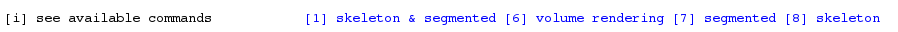
\includegraphics[scale=0.4]{fig/menu}

\section{Planes for different views}

\begin{figure}
	\centering
	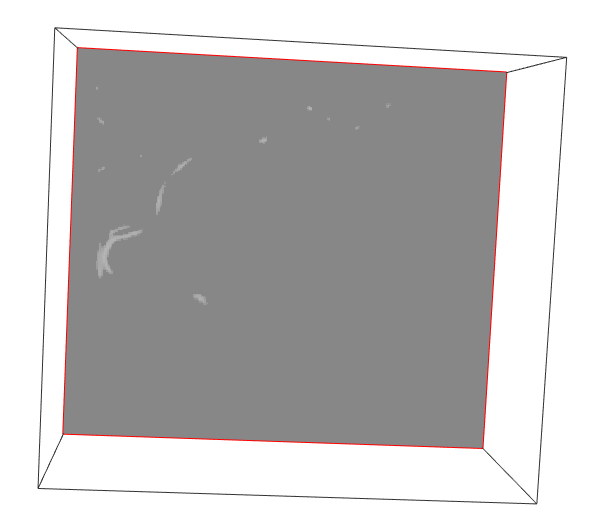
\includegraphics[scale=0.5]{fig/segmented-sagittal}
	\caption{Sagittal view for segmented image.}
	\label{fig:segmented-sagittal}
\end{figure}

A class vtkImagePlaneWidget was used to show the cut from the segmented data (Figure \ref{fig:segmented-sagittal}). In segmented image view we can show sagittal, transversal and coronal views by pressing keys S, T and C respectively. The segmented image is then hidden in order to show a cut and scrolling through the slices is possible by pressing + and - keys.

\section{Marching cubes and building the skeleton}


\section{Volume visualization}


\section{Point picker and distance calculation}


\section{Visualization}


\section{Using the Spline Widget}

